
\chapter{Description of the host structure}


\section{My position}

I did my internship in the University of Antwerp in the MSDL\footnote{Modelling, Simulation and Design Lab} laboratory. My stage chief was Prof. Hans Vangheluwe. But, because he is always busy and not always in the university for professional reason, I was attached to Simon Van Mierlo for this internship. He is a PhD student at the University of Antwerp. He works on the simulator of Statechart SCCD and he creates a debugger for this simulator.

Simon was chosen to be my tutor because first of all my work was very similar at a debugger interface and because Prof. Vangheluwe expected that I use SCCD as simulator and compare it with the simulator of Mr. Teodorov.

During my internship I work in the office of Simon and Yentl Van Tendeloo. But I was in relation with all members of MSDL.\footnote{It is possible to find a description of all MSDL members in \url{http://msdl.cs.mcgill.ca/people}}



\section{Position of MSDL}

\begin{figure}[h]
  \centering
  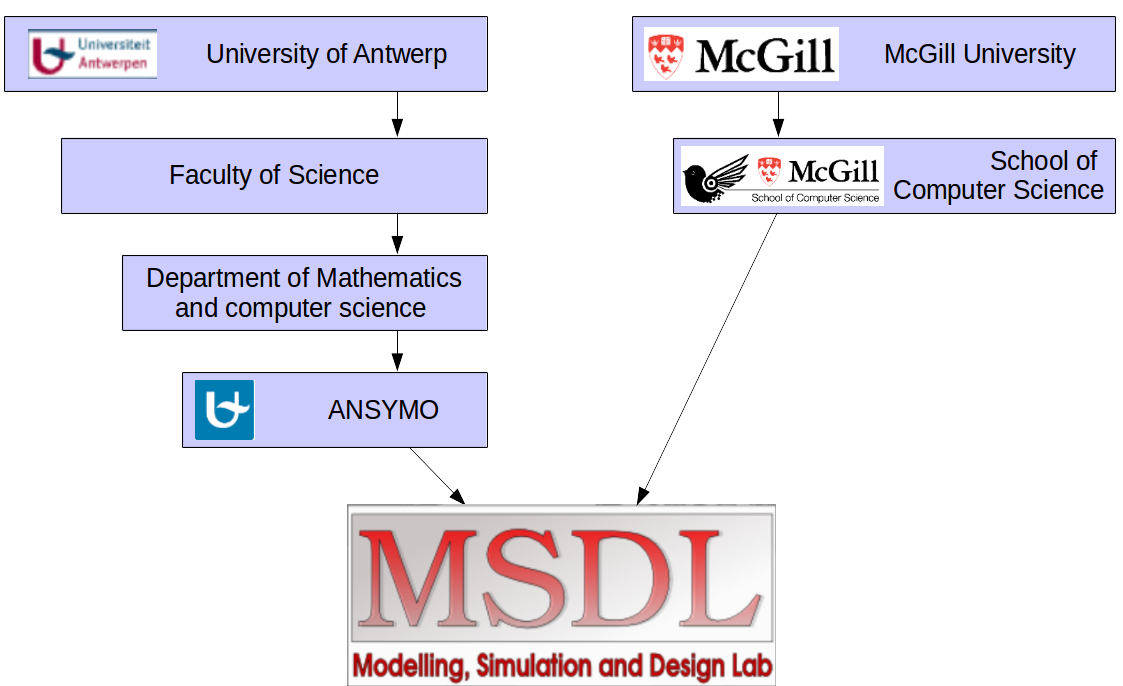
\includegraphics[width=0.8\linewidth]{msdl_organisation}

  \caption{Position of MSDL}
  \label{fig:msdl_org}
\end{figure}

The MSDL laboratory have members in two school, most part of these members are in the University of Antwerp but there is also some PhD students in the McGill University. McGill University is an English-language public research university in Montreal, Canada. You can see on the figure \ref{fig:msdl_org} a description of the organization of these universities\footnote{Only departments which belongs msdl were presented} and the position of MSDL in this organization.


\section{Description of MSDL}


\begin{figure}[!h]
  \centering
  
\includegraphics[width=0.6\textwidth]{MSDLbanner}
  \caption{MSDL banner}
  \label{fig:msdl}
\end{figure}


\begin{quotation}
<<The Modelling, Simulation and Design lab (MSDL) headed by Prof. Hans Vangheluwe is part of the School of Computer Science of McGill University in Montreal, Quebec, Canada and of the AnSyMo (Antwerp Systems and software Modelling) group in the department of Mathematics and Computer Science of the University of Antwerp, Antwerp, Belgium. The MSDL has projects, researchers and students in both locations.>>\cite{msdl}
\end{quotation}


So MSDL is a laboratory of Modeling. It is an important field of computer science because that could permit to create an engineering language understandable by everybody because it is based on graphical diagram. That also permit to create software without programming, just with logical diagram. I had the opportunity during my internship to participated in a presentation of all research subject. The figure \ref{fig:subject} is a not exhaustive list of all research topics discussed in MSDL. The part the most in connection with my subject was \textit{Simulation} and \textit{Analysis, Validation, Verification, Testing, and Accreditation} for obvious reasons.


\begin{figure}[h]
  \centering
  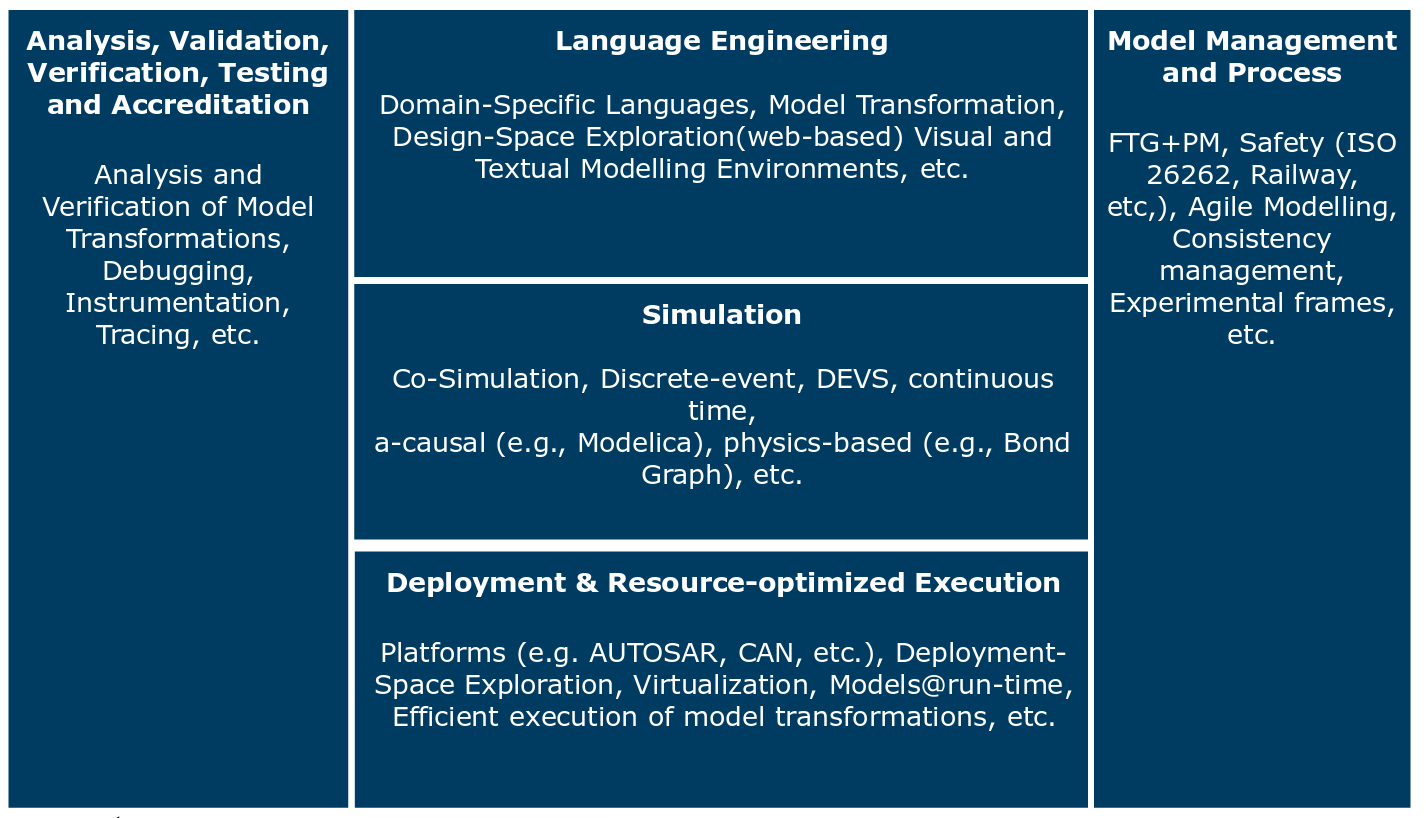
\includegraphics[width=\linewidth]{research}
  \caption{Research topics}
  \label{fig:subject}
\end{figure}



%%% Local Variables:
%%% mode: latex
%%% TeX-master: "../rapport_de_base"
%%% End:
